%% ut-thesis.tex -- document template for graduate theses at UofT
%%
%% Copyright (c) 1998-2013 Francois Pitt <fpitt@cs.utoronto.ca>
%% last updated at 16:20 (EDT) on Wed 25 Sep 2013
%%
%% This work may be distributed and/or modified under the conditions of
%% the LaTeX Project Public License, either version 1.3c of this license
%% or (at your option) any later version.
%% The latest version of this license is in
%%     http://www.latex-project.org/lppl.txt
%% and version 1.3c or later is part of all distributions of LaTeX
%% version 2005/12/01 or later.
%%
%% This work has the LPPL maintenance status "maintained".
%%
%% The Current Maintainer of this work is
%% Francois Pitt <fpitt@cs.utoronto.ca>.
%%
%% This work consists of the files listed in the accompanying README.

%% SUMMARY OF FEATURES:
%%
%% All environments, commands, and options provided by the `ut-thesis'
%% class will be described below, at the point where they should appear
%% in the document.  See the file `ut-thesis.cls' for more details.
%%
%% To explicitly set the pagestyle of any blank page inserted with
%% \cleardoublepage, use one of \clearemptydoublepage,
%% \clearplaindoublepage, \clearthesisdoublepage, or
%% \clearstandarddoublepage (to use the style currently in effect).
%%
%% For single-spaced quotes or quotations, use the `longquote' and
%% `longquotation' environments.


%%%%%%%%%%%%         PREAMBLE         %%%%%%%%%%%%

%%  - Default settings format a final copy (single-sided, normal
%%    margins, one-and-a-half-spaced with single-spaced notes).
%%  - For a rough copy (double-sided, normal margins, double-spaced,
%%    with the word "DRAFT" printed at each corner of every page), use
%%    the `draft' option.
%%  - The default global line spacing can be changed with one of the
%%    options `singlespaced', `onehalfspaced', or `doublespaced'.
%%  - Footnotes and marginal notes are all single-spaced by default, but
%%    can be made to have the same spacing as the rest of the document
%%    by using the option `standardspacednotes'.
%%  - The size of the margins can be changed with one of the options:
%%     . `narrowmargins' (1 1/4" left, 3/4" others),
%%     . `normalmargins' (1 1/4" left, 1" others),
%%     . `widemargins' (1 1/4" all),
%%     . `extrawidemargins' (1 1/2" all).
%%  - The pagestyle of "cleared" pages (empty pages inserted in
%%    two-sided documents to put the next page on the right-hand side)
%%    can be set with one of the options `cleardoublepagestyleempty',
%%    `cleardoublepagestyleplain', or `cleardoublepagestylestandard'.
%%  - Any other standard option for the `report' document class can be
%%    used to override the default or draft settings (such as `10pt',
%%    `11pt', `12pt'), and standard LaTeX packages can be used to
%%    further customize the layout and/or formatting of the document.

%% *** Add any desired options. ***
%\documentclass[twoside]{ut-thesis}


%%\newcommand{\myDocOptions}{10pt,twoside,openany,singlespaced,normalmargins,draft}

%% debug
%\newcommand{\myDocOptions}{11pt,a4,twoside,openany,singlespaced,normalmargins}
%\newcommand{\myDocOptions}{11pt,a4paper,oneside,openright,onehalfspaced,normalmargins}

%% production
\newcommand{\myDocOptions}{11pt,twoside,openright,onehalfspaced,normalmargins}


%\newcommand{\myDocOptions}{12pt,twoside,openany,oneandahalfspaced,normalmargins}
%\newcommand{\myDocOptions}{12pt,twoside,openany,doublespaced,normalmargins} %% ,draft}


\documentclass[\myDocOptions]{ut-thesis}




%% *** Add \usepackage declarations here. ***
%% The standard packages `geometry' and `setspace' are already loaded by
%% `ut-thesis' -- see their documentation for details of the features
%% they provide.  In particular, you may use the \geometry command here
%% to adjust the margins if none of the ut-thesis options are suitable
%% (see the `geometry' package for details).  You may also use the
%% \setstretch command to set the line spacing to a value other than
%% single, one-and-a-half, or double spaced (see the `setspace' package
%% for details).

\usepackage{url,alltt}
\usepackage{paralist, xspace}
\usepackage{caption}
\usepackage{subcaption}
\usepackage{graphicx}
\usepackage{wrapfig}
\usepackage{times}
\usepackage{amssymb,amsmath,pifont,footnote}
\usepackage{latexsym,pdfpages}
\usepackage{array,verbatim}
\usepackage{stmaryrd,ifsym}
\usepackage{algorithmic,algorithm}
\usepackage{gastex} % compile twice when pictures have changed.
\usepackage{parcolumns}
\usepackage{listings}
\usepackage{color}
\usepackage{hyperref}
\usepackage{cleveref}
\usepackage{enumitem}
\usepackage{amsthm}
\usepackage{pdfpages}


%%%%%%%%%%%%%%%%%%%%%%%%%%%%%%%%%%%%%%%%%%%%%%%%%%%%%%%%%%%%%%%%%%%%%%%%
%%                                                                    %%
%%                   ***   I M P O R T A N T   ***                    %%
%%                                                                    %%
%%  Fill in the following fields with the required information:       %%
%%   - \degree{...}       name of the degree obtained                 %%
%%   - \department{...}   name of the graduate department             %%
%%   - \gradyear{...}     year of graduation                          %%
%%   - \author{...}       name of the author                          %%
%%   - \title{...}        title of the thesis                         %%
%%%%%%%%%%%%%%%%%%%%%%%%%%%%%%%%%%%%%%%%%%%%%%%%%%%%%%%%%%%%%%%%%%%%%%%%

%% *** Change this example to appropriate values. ***
\degree{Master of Science}
\department{Computer Science}
\gradyear{2021}
\author{Peleg Kazaz}
\title{Communication Complexity of Set Disjointness Over Product Distributions}

%% *** NOTE ***
%% Put here all other formatting commands that belong in the preamble.
%% In particular, you should put all of your \newcommand's,
%% \newenvironment's, \newtheorem's, etc. (in other words, all the
%% global definitions that you will need throughout your thesis) in a
%% separate file and use "\input{filename}" to input it here.

\sloppy
%\pagestyle{empty}

\definecolor{dkgreen}{rgb}{0,0.6,0}
\definecolor{gray}{rgb}{0.5,0.5,0.5}
\definecolor{mauve}{rgb}{0.58,0,0.82}

\lstset{%frame=tb,
%  language=Java,
  %aboveskip=3mm,
  %belowskip=3mm,
  %showstringspaces=false,
  %columns=flexible,
  basicstyle={\small\ttfamily},
  %numbers=none,
%  basicstyle=\tiny,
%  numberstyle=\tiny\color{gray},
%  keywordstyle=\color{blue},
%  commentstyle=\color{dkgreen},
%  stringstyle=\color{mauve},
  %breaklines=true,
  %breakatwhitespace=true
%  tabsize=3
}
\setlist{nolistsep}



%\newtheorem{thm}{Theorem} %Added
%\newtheorem{notat}[thm]{Notations}
%%\newtheorem{lem}[thm]{Lemma}
%\newtheorem{lem}{Lemma}
%\newtheorem{WorkAround}{Lemma}
%%\newtheorem{prop}[thm]{Proposition}
%\newtheorem{prop}{Proposition}
%%\newtheorem{rem}[thm]{Remark}
%\newtheorem{rem}{Remark}
%\newtheorem{prob}{Problem}
%\newtheorem{fact}{Fact}
%
%%\newtheorem{cor}[thm]{Corollary}
%\newtheorem{cor}{Corollary}
%\newtheorem{Obs}{Observation}
%%\newenvironment{prop}{\theoremlike{Proposition}}{\par\medskip}
%%\theoremlike{prop}{<caption>}[<within>]
%%{\bfseries}{\itshape}
%%\newtheorem{defn}[thm]{Definition}
%\newtheorem{defn}{Definition}
%\newtheorem{examp}{Example}
%\newtheorem{example}{Example}
%%
%\newtheorem{dfn}[thm]{Definition}

%\newcommand{\pfbox}{\quad\hspace*{\fill}$\Box$}
%\newcommand{\pfbox}{\qed}

%\newenvironment{proof}{\noindent {\bf Proof}~}{\pfbox\bigskip}
% \renewcommand{\baselinestretch}{0.95}
%\renewcommand{\baselinestretch}{0.975}

% \setlength{\bibsep}{0.40ex}

\newcommand{\Nat}{\ensuremath{\mathbb{N}}}
\newcommand{\Rea}{\ensuremath{\mathbb{R}}}
\newcommand {\exptime} {\textsc{exptime}}
\def\Unbound{\mathit{Unbound}}
\def\Dense{\mathit{Dense}}
\def\blim{\mathit{base}-\lim}
\def\class{\mathcal{ C}}
\def\fF{\mathfrak{F}}
\def\clos{\mathit{Cl}}
\def\shuf{\mathit{shuffle}}
\def\fset{finite-set }
%\newcommand{\}{\mathit{Hin}}
\newcommand{\hin}{\mathit{Hin}}
\newcommand{\Flag}{\mbox{Updated}}
\newcommand{\false}{\mbox{False}}
\newcommand{\true}{\mbox{True}}
\newcommand{\TL}{\mathit{TL}}

\def\vp{\varphi}
\def\mG{\mathcal{G}}
\def\rar{\rightarrow}
\def\power{\mathcal{P}}
\def\s{\subseteq}
\def\All{\forall}
\def\we{\wedge}
\def\dep{\mathit{qd}}
\newcommand{\MLO}{\mbox{MLO}}
\newcommand{\FOMLO}{\mbox{FOMLO}}
\def\mL{\mathcal{L}}
\def\mM{\mathcal{M}}
\def\mR{\mathcal{R}}
\def\mI{\mathcal{I}}
\def\mJ{\mathcal{J}}
\def\mN{\mathcal{N}}
\def\MTh{\mathit{MTh}}
\def\HF{\mathit{type}}
\def\Th{\mathit{Th}}
\def\mD{\mathcal{D}}
\def\Form{\mathfrak{Form}}
\def\fS{\mathfrak{S}}
\def\fH{\mathfrak{H}}
\def\nek{\ldots}
\newcommand{\qd}[1]{\mathop{\rm qd}(#1)}
\def\strucmult{\otimes}
\def\typemult{\otimes}
\def\la{\lambda}
\def\close{\mathit{Closed}}
\def\win{\mathit{Win}}
\def\Realize{\mbox{Realize}}
\def\Dsynth{\mbox{Dsynth}}
\def\Fsynth{\mbox{Fsynth}}

\def\st{\mathit{st}}
\def\type{\mathit{type}}
\def\ttype{\mathit{ptype}}
\def\sgame{\mathit{Game}}
\def\res{\mathit{res}}
\def\win{\mathit{win}}
\def\Win{\mathit{Win}}
\def\Dwin{\mathit{Dwin}}
\def\Fswin{\mathit{Fswin}}
\def\Mult{\mathit{Mult}}
\newcommand{\G}[2]{R(#1,#2)}
\def\owin{\mbox{Or-win}}
\def\scaus{\mbox{I-Player-strategy}}
\def\caus{\mbox{II-Player-strategy}}
\def\upd{\mbox{next}}
\def\upl{\Delta}
\def\out{\mbox{out}}
\DeclareMathOperator{\rank}{rank}
\DeclareMathOperator{\weight}{weight}
\DeclareMathOperator{\col}{col}
\def\Dl{D^-}
\def\Dr{D^+}
\def\type{\mathit{type}}
\def\rest{\lfloor}
\def\dom{\partial}
\DeclareMathOperator{\Llim}{llim} \DeclareMathOperator{\Rlim}{rlim}
\def\aaut{\mathfrak{ A}}
\def\baut{\mathfrak{ B}}
\def\abasis{B}
\newcommand{\powerset}[1]{\mathcal{P}({#1})}
\newcommand{\arun}{\rho}
\newcommand{\AL}{{\rm always}}
\def\next{\mathit{next}}
\def\word{\mathit{s}}

\def\Left{\mathit{Left}}
\def\Right{\mathit{Right }}
\def\ovarphi{{\overline\varphi}}
\def\Neg{\mathit{Neg}}
\def\Id{\mathit{Id}}
\def\Conj{\mathit{Conj}}
\def\Disj{\mathit{Disj}}
\def\tr{\mathit{Tr}}
\def\diamonds{\overleftarrow{\diamondsuit}}
\newcommand{\LE}{\mbox{\it{Q2MLO}$_\exists$}}
\def\Lreg{\class_{reg}}
\def\lab{\mathit{lab}}
\def\Rreg{\mR_{reg}}

\def\One{\mathit{One}}

\newcommand{\simplies}{\DOTSB\Longrightarrow}

%\newif\iffullproofs
%\newif\ifshortproofs
%\newif\iflong
%\newif\iftacas


%%%% for tacas use:
% \fullproofsfalse
% \shortproofstrue
% \longfalse
% \tacastrue

%%%% for tech report use
% \fullproofsfalse
% \shortproofstrue
% \longfalse
% \tacasfalse


%%\proofstrue
%% short version
%\fullproofsfalse
%\shortproofstrue
%\longfalse
%\tacastrue

% % long version
% \fullproofstrue
% \shortproofsfalse
% \longtrue


\newtheorem{theorem}{Theorem}
\newtheorem{remark}{Remark}
\newtheorem{lemma}[theorem]{Lemma}
\newtheorem{claim}[theorem]{Claim}
\newtheorem{conjecture}[theorem]{Conjecture}
\newtheorem{corollary}[theorem]{Corollary}
\newtheorem{fact}[theorem]{Fact}
\newtheorem{proposition}[theorem]{Proposition}
\newtheorem{problem}[theorem]{Problem}
\newtheorem{observation}[theorem]{Observation}
\newtheorem{definition}[theorem]{Definition}
\newtheorem{requirement}[theorem]{Requirement}
\newtheorem{example}[theorem]{Example}
%\newenvironment{proof}[1][Proof]{\begin{trivlist}
%\item[\hskip \labelsep {\bfseries #1}]}
%{\end{trivlist}
%\qed
%}


\newcommand{\exref}[1]{Example~\ref{examp:#1}}
\newcommand{\chapref}[1]{Chapter~\ref{chap:#1}}
\newcommand{\secref}[1]{Section~\ref{sec:#1}}
\newcommand{\lemref}[1]{Lemma~\ref{lem:#1}}
\newcommand{\remref}[1]{Remark~\ref{rem:#1}}
\newcommand{\figref}[1]{Figure~\ref{Fi:#1}}
\newcommand{\thmref}[1]{Theorem~\ref{thm:#1}}
\newcommand{\gV}[1]{\langle \textit{#1}\rangle}
\newcommand{\bid}{\textbf{id}}
\newcommand{\brcv}{\textbf{input}}
\newcommand{\breceive}{\brcv}
\newcommand{\bfrw}{\textbf{output}}
\newcommand{\bforward}{\bfrw}
\newcommand{\bto}{\textbf{to}}
\newcommand{\bif}{\textbf{if}}
\newcommand{\bthen}{\textbf{then}}
\newcommand{\belse}{\textbf{else}}
\newcommand{\binsert}{\textbf{insert}}
\newcommand{\bremove}{\textbf{remove}}
\newcommand{\babort}{\textbf{abort}}
\newcommand{\bskip}{\textbf{skip}}
\newcommand{\bfor}{\textbf{for}}
\newcommand{\bforall}{\textbf{forall}}
\newcommand{\bin}{\textbf{in}}
\newcommand{\band}{\textbf{and}}
\newcommand{\bor}{\textbf{or}}
\newcommand{\bnot}{\textbf{not}}
\newcommand{\bself}{\textbf{self}}
\newcommand{\btuple}[1]{\overline{#1}}
% Learning Switch
\newcommand{\tconnected}{\texttt{connected}}
\newcommand{\tallPorts}{\texttt{allPorts}}
% Firewall
\newcommand{\ttrusted}{\texttt{trusted}}
% Proxy
\newcommand{\tcache}{\texttt{cache}}
\newcommand{\tresponse}{\texttt{response}}
\newcommand{\trequested}{\texttt{requested}}
% Isolation
\newcommand{\tforbidden}{\texttt{forbidden}}
\newcommand{\authorComment}[2]{\textbf{#1:}{\textit{#2}}}
\newcommand{\MVer}{\texttt{MuteVeri}}
\newcommand{\N}{\mathbb{N}}
\newcommand{\authorNote}{}
% Round-Robin
\newcommand{\tnextport}{\texttt{nextport}}

\newcommand{\bdo}{\textbf{do}}
\newcommand{\bwhile}{\textbf{while}}
\newcommand{\bforeach}{\textbf{foreach}}
\newcommand{\breturn}{\textbf{return}}
\newcommand\scalemath[2]{\scalebox{#1}{\mbox{\ensuremath{\displaystyle #2}}}}



%%%% Macros from main

\newcommand{\TODO}[1]{{\color{red} \textit{ \textbf{ TODO: #1 }}}}


\newcommand{\tuple}[1]{\left(#1\right)}
\newcommand{\bliml}{\mathit{Base}_{\underrightarrow{\lim }} }
\newcommand{\blimr}{\mathit{Base}_{\underleftarrow{\lim }} }
\def\set#1{\{ #1 \}}
\def\th{\lambda}

\newcommand{\SC}{\mathcal{SFOT_{\cA}}}
\newcommand{\ub}{\mathit{ub}}
%\newcommand{\Set}[1]{\{ #1 \}}

\newcommand{\sft}{\mathcal{SFOT}_{n}}
\newcommand{\cA}{\mathcal{A}}
\newcommand{\cC}{\mathcal{C}}
\newcommand{\cL}{\mathcal{L}}
\newcommand{\cI}{\mathcal{I}}
\newcommand{\wi}{\mathit{Win_{I}}}
\newcommand{\McN}{\mathit{McNGame}}
\newcommand{\cB}{\mathcal{B}}
\newcommand{\cond}{FOT }
\newcommand{\ra}{\rightarrow}
\newcommand{\lar}{\leftarrow}
\newcommand{\Ps}[1]{\mathbb{P}( #1 )}
\newcommand{\gt}{\mbox{game-type}}
\newcommand{\code}{\mbox{Code}}
\newcommand{\trun}{\mbox{trun}}
\newcommand{\gcode}{\mbox{gcode}}
\newcommand{\Play}{\mbox{Play}}
\newcommand{\nat}{\mathbb{N}}
\newcommand{\Z}{\mathbb{Z}}
\newcommand{\Q}{\mathbb{Q}}
\newcommand{\R}{\mathbb{R}}
\newcommand{\mcT}{\mathcal{T}}
\newcommand{\om}{\omega}

% Yaronv new commands
\newcommand{\PlusMinus}{+-}
\newcommand{\Set}[1]{\{ #1 \}}
\newcommand{\Range}[2]{#1 ,\dots, #2}
\newcommand{\RangeSet}[2]{\Set{ \Range{#1}{#2}}}
\newcommand{\EC}{\mathit{EC}}
\newcommand{\ER}{\mathit{ER}}
\newcommand{\Interp}{\mathit{Interp}}
\newcommand{\PSR}[1]{\ensuremath{\mathit{PSR}(#1)}}
\newcommand{\DE}[1]{\textrm{DE}_{#1}}
\newcommand{\UDE}[1]{\textrm{UDE}_{#1}}
\newcommand{\DEfin}{\ensuremath{ \textrm{{DE}}_{\mathit{fin}}   }    }
\newcommand{\UDEfin}{\ensuremath{ \textrm{{UDE}}_{\mathit{fin}}   }    }

\newcommand{\BeginMultiCycle}{\overrightarrow{\mathfrak{m}}}
\newcommand{\EndMultiCycle}{\overleftarrow{\mathfrak{m}}}
\newcommand{\BeginCycle}{\overrightarrow{\mathfrak{c}}}
\newcommand{\EndCycle}{\overleftarrow{\mathfrak{c}}}

\newcommand{\highz}{\ensuremath{z}}
\newcommand{\E}[1]{\textrm{E}_{#1}}
\newcommand{\Efin}{\ensuremath{ \textrm{{E}}_{\mathit{fin}}   }    }
\newcommand{\MSO}{\textrm{MSO}}
\newcommand{\Couple}[2]{\ensuremath{\binom{#2}{#1}}}
\newcommand{\SigLetter}[2]{\ensuremath{\sigma_{#1}(#2)}}
\newcommand{\SigLetterOne}[1]{\ensuremath{\SigLetter{1}{#1}}}
\newcommand{\SigLetterTwo}[1]{\SigLetter{2}{#1}}
\newcommand{\SigTuple}[1]{\Couple{\SigLetterOne{#1}}{ \SigLetterTwo{#1} } }
\newcommand{\sigTuple}{\Couple{\sigma_1}{ \sigma_2 } }
\newcommand{\SigmaMult}{\ensuremath{\Sigma_1 \times \Sigma_2}}
\newcommand{\SigmaMultOmega}{\ensuremath{(\SigmaMult)^\omega}}
\newcommand{\SigmaEps}{\ensuremath{\Sigma_1 \cup \singelton{\highz}}}
\newcommand{\SigmaEpsMult}{\ensuremath{(\SigmaEps) \times \Sigma_2}}
\newcommand{\SigmaEpsMultOmega}{\ensuremath{(\SigmaEpsMult)^\omega}}
\newcommand{\GameGraph}[1]{\langle #1 \rangle}
\newcommand{\Tuple}[1]{\langle #1 \rangle}
\newcommand{\WtFunc}{\mathit{wt}}
\newcommand{\QDeadEnd}{ \ensuremath{ q_{\mbox{dead-end}} } }
\newcommand{\MPSupGeq}[1]{\ensuremath{\textrm{MeanPayoffSup}^{\geq}(#1)}}
\newcommand{\MPSupGt}[1]{\ensuremath{\textrm{MeanPayoffSup}^{>}(#1)}}
\newcommand{\MPSupGeneric}[1]{\ensuremath{\textrm{MeanPayoffSup}^{\sim}(#1)}}
\newcommand{\MPInfGeneric}[1]{\ensuremath{\textrm{MeanPayoffInf}^{\sim}(#1)}}
\newcommand{\MPSupBoth}[1]{\ensuremath{\textrm{MeanPayoffSup}^{\geq, >}(#1)}}
\newcommand{\MPInfBoth}[1]{\ensuremath{\textrm{MeanPayoffInf}^{\geq, >}(#1)}}
\newcommand{\MPSupGenericIndexed}[2]{\ensuremath{\textrm{MeanPayoffSup}^{\sim_{#2}}(#1)}}
\newcommand{\MPInfGenericIndexed}[2]{\ensuremath{\textrm{MeanPayoffInf}^{\sim_{#2}}(#1)}}
\newcommand{\MPSupLeq}[1]{\ensuremath{\textrm{MeanPayoffSup}^{\leq}(#1)}}
\newcommand{\MPInfGeq}[1]{\ensuremath{\textrm{MeanPayoffInf}^{\geq}(#1)}}
\newcommand{\MPInfGt}[1]{\ensuremath{\textrm{MeanPayoffInf}^{>}(#1)}}
\newcommand{\MPInfLeq}[1]{\ensuremath{\textrm{MeanPayoffInf}^{\leq}(#1)}}
\newcommand{\MPInfLt}[1]{\ensuremath{\textrm{MeanPayoffInf}^{<}(#1)}}
\newcommand{\EL}[1]{\ensuremath{\mathit{EL}(#1)}}
\newcommand{\MPSup}{\ensuremath{ \overline{\mathit{MP}}}}
\newcommand{\MPInf}{\ensuremath{ \underline{\mathit{MP}}}}
\newcommand{\OrMP}{\ensuremath{O^{\textrm{MP}}}}
\newcommand{\AttrOne}[1]{\ensuremath{Attr_1(#1)}}
\newcommand{\AttrTwo}[1]{\ensuremath{Attr_2(#1)}}
\newcommand{\AttrOneG}[2]{\ensuremath{Attr_1^{#1}(#2)}}
\newcommand{\AttrTwoG}[2]{\ensuremath{Attr_2^{#1}(#2)}}
\newcommand{\Attri}[1]{\ensuremath{Attr_i(#1)}}
\newcommand{\Automat}[1]{\ensuremath{\mathcal{#1}}}

\newcommand{\ConjMPSupGeq}[1]{\ensuremath{\bigwedge\MPSupGeq{#1}}}
\newcommand{\ConjMPSupGenericIndexed}[2]{\ensuremath{\bigwedge\MPSupGenericIndexed{#1}{#2}}}
\newcommand{\ConjMPSupGt}[1]{\ensuremath{\bigwedge\MPSupGt{#1}}}
\newcommand{\ConjMPInfGeq}[1]{\ensuremath{\bigwedge\MPInfGeq{#1}}}
\newcommand{\ConjMPInfGt}[1]{\ensuremath{\bigwedge\MPInfGt{#1}}}
\newcommand{\ConjMPInfGenericIndexed}[2]{\ensuremath{\bigwedge\MPInfGenericIndexed{#1}{#2}}}
\newcommand{\ConjMPInfSupGeq}[2]{\ensuremath{\bigwedge\textrm{MeanPayoffInf}^{\geq}_{#2}(#1)\wedge\bigwedge\textrm{MeanPayoffSup}^{\geq}_{#2 ^c}(#1)}} \newcommand{\ConjMPInfSupGt}[2]{\ensuremath{\bigwedge\textrm{MeanPayoffInf}^{>}_{#2}(#1)\wedge\bigwedge\textrm{MeanPayoffSup}^{>}_{#2 ^c}(#1)}}

\newcommand{\ConjDisjMPSupGeq}[1]{\ensuremath{\bigwedge\bigvee\MPSupGeq{#1}}}
\newcommand{\DisjConjMPInfGeq}[1]{\ensuremath{\bigvee\bigwedge\MPInfGeq{#1}}}
\newcommand{\ConjDisjMPSupGt}[1]{\ensuremath{\bigwedge\bigvee\MPSupGt{#1}}}
\newcommand{\DisjConjMPInfGt}[1]{\ensuremath{\bigvee\bigwedge\MPInfGt{#1}}}
\newcommand{\ConjDisjMPSupBoth}[1]{\ensuremath{\bigwedge\bigvee\MPSupBoth{#1}}}
\newcommand{\DisjConjMPInfBoth}[1]{\ensuremath{\bigvee\bigwedge\MPInfBoth{#1}}}



\newcommand{\Heading}[1]{\vspace{-0.3cm}\paragraph{{#1}}}
\newcommand{\BeginProof}{\vspace{-0.25cm}\begin{proof}}
\newcommand{\PreSection}{\vspace{-0.5cm}}
\newcommand{\PostSection}{\vspace{-0.0cm}}


%\newcommand{\Heading}[1]{\noindent\textbf{#1}}
\newcommand{\PreItemize}{\vspace{-0.1cm}}
\newcommand{\PostItemize}{\vspace{-0.1cm}}

\newcommand{\ProofOutline}[1]{\paragraph{\bf{A proof outline for {#1}}}}
%\newcommand(\PreSection}{\vspace{-0.25cm}}
%\newcommand(\EndSection}{\vspace{-0.25cm}}


\newcommand{\ADD}{{\sc Add}}
\newcommand{\GET}{{\sc Get}}
\newcommand{\DEL}{{\sc Delete}}

\newcommand{\method}[1]{\textbf{#1}}
\newcommand{\container}[1]{\textbf{#1}}
%\newcommand{\linecode}[1]{\textbf{$#1$}}


\newcommand{\Comment}[1]{}
\newcommand{\Appendix}[1]{}

\newcommand{\MAX}{\max}
\newcommand{\MIN}{\min}
\newcommand{\SUM}{\operatorname{sum}}
\newcommand{\OP}{\operatorname{op}}
\newcommand{\Avg}{\mathit{Avg}}
\newcommand{\LimInfAvg}{\mathit{LimInfAvg}}
\newcommand{\LimSupAvg}{\mathit{LimSupAvg}}
\newcommand{\LimSupAvgAutomat}[1]{\overline{#1}}
\newcommand{\LimInfAvgAutomat}[1]{\underline{#1}}
\newcommand{\LimRatio}{\mathit{LimRat}}
\newcommand{\LimAvg}{\mathit{LimAvg}}
\newcommand{\Rat}{\mathit{Rat}}


\newcommand{\NoMax}{\mathit{NoMax}}

\newcommand{\InfAvgLan}[2]{\underline{#1}^{\geq #2}}
\newcommand{\SupAvgLan}[2]{\overline{#1}^{\geq #2}}

\newcommand{\MultiCycle}[1]{\mathbf{#1}}
\newcommand{\VEC}[1]{\ensuremath{\overline{#1}}}

\newcommand{\ProofOfRem}[1]{of Remark \ref{#1}}
\newcommand{\ProofOfThm}[1]{of Theorem \ref{#1}}
\newcommand{\ProofOfLem}[1]{of Lemma \ref{#1}}
\newcommand{\ProofOfProp}[1]{of Proposition \ref{#1}}
\newcommand{\ProofOfCor}[1]{of Corollary \ref{#1}}
\newcommand{\ProofOfObs}[1]{of Observation \ref{#1}}



\newcommand{\until}{{\sf Until}}
\newcommand{\since}{{\sf Since}}
\newcommand{\ltl}{{\rm LTL}}
\newcommand {\pspace} {\textsc{pspace}}
\newcommand{\mainlogic}{\TL(\until,\since)}


\newcommand{\CMPSup}{\ensuremath{\bigwedge \textrm{MeanPayoffSup} }}
\newcommand{\CMPInf}{\ensuremath{\bigwedge \textrm{MeanPayoffInf} }}
\newcommand{\DMPSup}{\ensuremath{\bigvee \textrm{MeanPayoffSup} }}
%\newcommand{\SPAN}{\operatorname{SPAN}}
%\newcommand{\SPANge}{\operatorname{SPAN}^{\geq}}
%\newcommand{\SMPO}{\operatorname{SMPO}}

\newcommand{\DMPInf}{\ensuremath{\bigvee \textrm{MeanPayoffInf} }}

\newcommand{\MinExpVal}[2]{\ensuremath{\min_{#2} {#1}}}
\newcommand{\Floor}[2]{\ensuremath{\lfloor{#1}\rfloor_\frac{1}{#2}}}

\newcommand{\Char}{\operatorname{characterization}}
\newcommand{\EChar}{\operatorname{ECP}}
\newcommand{\SCC}{\operatorname{SCC}}
\newcommand{\Cycle}{\operatorname{Cycle}}
\newcommand{\SPAN}{\mathit{SPAN}}
\newcommand{\UCSPAN}{\mathit{UCSPAN}}
\newcommand{\DCSPAN}{\mathit{DCSPAN}}
\newcommand{\RelRatSPAN}{\mathit{relRatSPAN}}
\newcommand{\RelSPAN}{\mathit{relSPAN}}
\newcommand{\UC}{\mathit{UC}}
\newcommand{\DC}{\mathit{DC}}
\newcommand{\SPANGame}{\ensuremath{\mathit{LSMMP}}}
\newcommand{\UCGGame}{\ensuremath{\mathit{UCG}}}
\newcommand{\SimpleConnectedReachable}{\ensuremath{\mathit{SCR}}}

\newcommand{\Val}{\ensuremath{\mathit{Val}}}
\newcommand{\ValP}{\ensuremath{\mathit{Val}^{\mathit{worst}}}}
\newcommand{\ValO}{\ensuremath{\mathit{Val}^{\mathit{best}}}}
\newcommand{\FM}{\mathcal{FM}}

\newcommand{\MinThresh}{\mathit{MT}}
\newcommand{\RelaxedMinThresh}{\mathit{RMT}}
\newcommand{\OPT}{\mathit{OPT}}

\newcommand{\AppendixString}{\cite{mpexpressionCorr}}
\newcommand{\AppendixContent}[1]{}

\newcommand{\MPG}{\mathit{MPG}}
\newcommand{\NULL}{\mathit{NULL}}
\newcommand{\Parent}{\mathit{parent}}
\newcommand{\Ack}{\mathit{ACK}}
\newcommand{\Name}{\newpage Yaron Velner 043245810 (assignment 3)}
%\newcommand{\Name}{}

\newcommand{\En}{\mathit{En}}
\newcommand{\Ex}{\mathit{Ex}}
\newcommand{\Calls}{\mathit{Calls}}
\newcommand{\Retns}{\mathit{Retns}}
\newcommand{\InvRetns}{\mathit{Retns}^{-1}}
\newcommand{\RSM}{\mathit{ICFG}}
\newcommand{\QRSM}{\mathit{QICFG}}
\newcommand{\wrg}{\mathcal{A}}
\newcommand{\Good}{\mathit{good}}
\newcommand{\Bad}{\mathit{bad}}
\newcommand{\Neutral}{\mathit{neutral}}





\def\Skip{\mathit{skip}}
\def\Pop{\mathit{pop}}
\def\Push{\mathit{push}}
\def\Com{\mathsf{Com}}
\def\com{\mathit{com}}
\newcommand{\SH}{\mathsf{SH}}
\newcommand{\ASH}{\mathsf{ASH}}
\newcommand{\Top}{\mathsf{Top}}

\newcommand{\Gr}{\mathsf{Gr}}

\newcommand{\Compact}{\mathsf{Comp}}

\newcommand{\Rank}{\mathsf{Rank}}
\newcommand{\ie}{{\it i.e.,}\xspace}
\newcommand{\eg}{{\it e.g.,}\xspace}
\newcommand\eat[1]{}

%%%%%%%%%%%%%  new definitions for AMDL
\newcommand{\Net}{\mathsf{N}}
\newcommand{\PortSet}{\mathsf{Pr}}
\newcommand{\SinglePort}{\mathit{pr}}
\newcommand{\ForwardFunc}{\mathsf{f}}
\newcommand{\ForwardRel}{\mathsf{f_r}}
\newcommand{\Channel}{\mathsf{C}}
\newcommand{\IngChannel}{\mathsf{C_{\mathit{ingress}}}}
\newcommand{\EgChannel}{\mathsf{C_{\mathit{egress}}}}
\newcommand{\allnotes}[1]{}
% To make the FIXMEs go away, comment out this line...
\renewcommand{\allnotes}[1]{\textit{#1}}
\newcommand{\fixme}[1]{\allnotes{\bf\textcolor{red}{[#1]}}}
\newcommand{\notepanda}[1]{\allnotes{\textcolor{blue}{[Panda: #1]}}}
%\newcommand{\Name}{}

%\newcommand{\AbsPackets}{{P^{\sharp}}}
\newcommand{\AbsPackets}{{P}}

%\newcommand{\abortstate}{\bot}




%% *** Adjust the following settings as desired. ***

%% List only down to subsections in the table of contents;
%% 0=chapter, 1=section, 2=subsection, 3=subsubsection, etc.
\setcounter{tocdepth}{2}

%% Make each page fill up the entire page.
\flushbottom


%%%%%%%%%%%%      MAIN  DOCUMENT      %%%%%%%%%%%%

\begin{document}

%% This sets the page style and numbering for preliminary sections.
\begin{preliminary}

%% This generates the title page from the information given above.
\maketitle

%% There should be NOTHING between the title page and abstract.
%% However, if your document is two-sided and you want the abstract
%% _not_ to appear on the back of the title page, then uncomment the
%% following line.
\cleardoublepage

%% This generates the abstract page, with the line spacing adjusted
%% according to SGS guidelines.
\begin{abstract}
Lorem ipsum dolor sit amet, consectetur adipiscing elit. In maximus tellus eget erat congue cursus. Donec nulla dui, pretium at euismod ultrices, dictum quis mauris. Maecenas accumsan gravida elit cursus elementum. Nunc euismod mauris et tincidunt faucibus. Integer dolor quam, vulputate sed odio id, ornare mattis mi. In iaculis efficitur tortor, quis fermentum dolor blandit et. Vivamus tempor rutrum turpis vitae elementum. Morbi fermentum nulla a iaculis ultricies. Cras dictum dapibus odio, in fermentum justo porta quis. Donec a neque diam. Ut convallis sodales blandit.

Integer nec nibh eget erat eleifend condimentum in sit amet odio. Integer justo elit, tempus eget ultricies vel, congue eget sem. Curabitur augue nibh, dignissim at rhoncus pulvinar, gravida sit amet ante. Aenean ullamcorper velit id nulla porta cursus. Proin placerat urna quis metus egestas congue. Donec posuere leo eget sapien imperdiet, ultricies volutpat arcu tincidunt. Morbi egestas magna a nisi sagittis, nec elementum ex tincidunt. Nunc euismod dui leo, ut viverra nulla commodo ut. In sed sem et ligula fermentum mollis sit amet in tellus. Nam ac neque neque. Nunc lacinia nibh lectus, sit amet dictum libero tempor in.

Nunc malesuada eros vel purus lobortis sollicitudin. Nam in viverra nunc. Duis tincidunt velit diam, et sodales augue posuere sed. Ut cursus metus et arcu fermentum, id imperdiet ipsum interdum. Nullam eleifend non tellus eget semper. In dictum consequat enim, eget auctor lacus volutpat et. Vestibulum in urna mauris. In hac habitasse platea dictumst. Phasellus tempus eros placerat, tincidunt orci at, hendrerit felis. Class aptent taciti sociosqu ad litora torquent per conubia nostra, per inceptos himenaeos. Mauris ac lacinia justo, a lobortis odio. 
\end{abstract}
%\begin{abstract}
%% *** Put your Abstract here. ***
%% (At most 150 words for M.Sc. or 350 words for Ph.D.)
%\end{abstract}

%% Anything placed between the abstract and table of contents will
%% appear on a separate page since the abstract ends with \newpage and
%% the table of contents starts with \clearpage.  Use \cleardoublepage
%% for anything that you want to appear on a right-hand page.

\cleardoublepage
%% This generates a "dedication" section, if needed -- just a paragraph
%% formatted flush right (uncomment to have it appear in the document).
%\begin{dedication}
%\end{dedication}

%% The `dedication' and `acknowledgements' sections do not create new
%% pages so if you want the two sections to appear on separate pages,
%% uncomment the following line.
%\newpage  % separate pages for dedication and acknowledgements

%% Alternatively, if you leave both on the same page, it is probably a
%% good idea to add a bit of extra vertical space in between the two --
%% for example, as follows (adjust as desired).
%\vspace{.5in}  % vertical space between dedication and acknowledgements

\cleardoublepage
%% This generates an "acknowledgements" section, if needed
%% (uncomment to have it appear in the document).
\begin{acknowledgements}
%% *** Put your Acknowledgements here. ***
Lorem ipsum dolor sit amet, consectetur adipiscing elit. Nam pharetra tellus sit amet dolor vulputate aliquam at vitae magna. Maecenas imperdiet lobortis urna et egestas. Nullam iaculis nulla id nibh viverra, et aliquam dui tincidunt. Vestibulum viverra sodales lectus a luctus. Phasellus mattis, sapien in euismod imperdiet, ex augue consequat libero, eget suscipit lorem ligula sed orci. Proin rhoncus lacinia faucibus. Quisque maximus odio non metus ullamcorper facilisis. Pellentesque nibh leo, fermentum vel cursus eget, fringilla aliquam arcu. Interdum et malesuada fames ac ante ipsum primis in faucibus. Aenean maximus lobortis mi, ac porta libero viverra vel.

Morbi mattis, orci in aliquet dapibus, urna odio commodo libero, ut consequat leo arcu in libero. Aliquam dapibus sem justo. Praesent vel rhoncus lectus. Fusce sit amet turpis cursus mi dictum vulputate. Nullam consequat commodo quam, quis dignissim ligula tempor quis. In cursus enim nulla, efficitur aliquam nisl consectetur quis. Vivamus cursus iaculis accumsan. Integer nibh quam, semper at urna id, condimentum imperdiet lectus. Donec molestie sem metus, non placerat tortor malesuada a. Duis non ipsum luctus, lobortis leo sed, feugiat tortor. Suspendisse ut eros non justo pellentesque semper. Nunc felis mauris, interdum eu mattis eget, maximus ac massa. Pellentesque a elementum elit, vitae facilisis ipsum. Aenean sit amet suscipit eros. 
\end{acknowledgements}

%% This generates the Table of Contents (on a separate page).
\tableofcontents

%% This generates the List of Tables (on a separate page), if needed
%% (uncomment to have it appear in the document).
%\listoftables

%% This generates the List of Figures (on a separate page), if needed
%% (uncomment to have it appear in the document).
%\listoffigures

%% You can add commands here to generate any other material that belongs
%% in the head matter (for example, List of Plates, Index of Symbols, or
%% List of Appendices).

%% End of the preliminary sections: reset page style and numbering.
\end{preliminary}


%%%%%%%%%%%%%%%%%%%%%%%%%%%%%%%%%%%%%%%%%%%%%%%%%%%%%%%%%%%%%%%%%%%%%%%%
%%  Put your Chapters here; the easiest way to do this is to keep     %%
%%  each chapter in a separate file and `\include' all the files.     %%
%%  Each chapter file should start with "\chapter{ChapterName}".      %%
%%  Note that using `\include' instead of `\input' will make each     %%
%%  chapter start on a new page, and allow you to format only parts   %%
%%  of your thesis at a time by using `\includeonly'.                 %%
%%%%%%%%%%%%%%%%%%%%%%%%%%%%%%%%%%%%%%%%%%%%%%%%%%%%%%%%%%%%%%%%%%%%%%%%

\chapter{Introduction}
\section{Introduction}
\label{sec:intro}

In his seminal '79 paper introducing the notion of two-party communication complexity~\cite{Yao79},
Yao also briefly considered communication between more than two players, and pointed out ``one situation that deserves special attention'': two players receive private inputs, and send randomized messages to a third player, who then produces the output.
Yao asked what is the communication complexity of the Equality function (called ``the identification function'' in~\cite{Yao79}) in this model:
in 
the Equality function $\EQ_n$, the two players receive vectors $\set{0,1}^n$, and the goal is to determine whether $x = y$.


Yao showed in~\cite{Yao79} that $\EQ_n$ requires $\Omega(n)$ bits for determistic communication protocols, even if the players can communicate back-and-forth. Using a \emph{shared} random string, the complexity reduces to $O(1)$, and using \emph{private} randomness, but more than a single round, the complexity is $\Theta(\log n)$. In modern nomenclature, the model described above is called \emph{the 2-player simultaneous model}, and the third player (who announces the output) is called the \emph{referee}. Yao's question is then: what is the communication complexity of $\EQ_n$ using private randomness in the simultaneous model of communication complexity?

Some seventeen years later, Yao's question was answered: Newman and Sezegy showed in~\cite{NS96} that $\EQ_n$ requires $\Theta(\sqrt{n})$ bits to compute in the model above, if the players are allowed only private randomness. (Using shared randomness the complexity reduces to $O(1)$, even for simultaneous protocols.) Moreover, Babai and Kimmel showed in~\cite{BK97} that for \emph{any} function $f$, if the deterministic simultaneous complexity of $f$ is $D(f)$, then the private-coin simultaneous communication complexity of $f$ is $\Omega(\sqrt{D(f)})$, so in this sense private randomness is of only limited use for simultaneous protocols.

In this work we study multi-player simultaneous communication complexity%
\footnote{We consider the \emph{number-in-hand} model, where each player receives a private input, rather than the perhaps
more familiar \emph{number-on-forehead} model, where each player can see the input of all the other players but not its own.}%
, and ask: how useful are private random coins for more than two players? Intuitively, one might expect that as the number of players grows, the utility of private randomness should decrease.
%
%In particular, several 2-player protocols for $\EQ_n$~\cite{BK97,NS96} achieve communication complexity of $\tilde{O}(\sqrt{n})$ by relying on the \emph{birthday paradox}, which allows the two players to privately each select $\Theta(\sqrt{n})$ random objects from a universe of size $\Theta(n)$ --- and have constant probability that the same object will be selected by both players. For more than two players, we would need $\omega(\sqrt{n})$ random choices from each player --- as the number of players goes to infinity, the number of random choices required to ensure a global intersection approaches the size of the universe. Thus, it might seem that as the number of players goes to infinity, the private-coin simultaneous communication complexity of a function should much closer to its deterministic simultaneous complexity, and perhaps even the two should converge in the limit.
%
We first extend the $\Omega(\sqrt{D(f)})$ lower bound of~\cite{BK97} to the multi-player setting, and show that for any $k$-player function $f$,
the private-coin simultaneous communication complexity of $f$ is $\Omega(\sqrt{D(f)})$.
We then show, perhaps contrary to expectation, that the extended lower
bound is still tight in some cases.

To see why this may be surprising, consider the function $\AllEQ_{k,n}$, which generalizes $\EQ_n$ to $k$ players: each player $i$ receives a vector $x_i \in \set{0,1}^n$, and the goal is to determine whether all players received the same input. It is easy to see that the deterministic communication complexity of $\AllEQ_{k,n}$ is $\Omega(nk)$ (not just for simultanoues protocols), and each player must send $n$ bits to the referee in the worst case. From the lower bound above, we obtain a lower bound of $\Omega(\sqrt{nk})$ for the private-coin simultaneous complexity of $\AllEQ_{k,n}$.
It is easy to see that $\Omega(k)$ is also a lower bound, as each player must send at least one bit, so together we have a lower bound of $\Omega(\sqrt{nk}+k)$.
If this lower bound is tight, then the average player only needs to send $O(\sqrt{n/k}+1)$ bits to the referee in the worst-case, so in some sense we even \emph{gain} from having more players, and indeed, if $k = \Omega(n)$, then the per-player cost of $\AllEQ_{k,n}$ with private coins is constant, just as it would be with shared coins.

Nevertheless, our lower bound \emph{is} nearly tight, and we are able to give a simultaneous private-coin protocol for $\AllEQ_{k,n}$ where each players sends only $O(\sqrt{n/k} + \log(k))$ bits to the referee,
for a total of $O(\sqrt{nk}+ k \log \min \set{ k, n})$ bits.
This matches the lower bound of $\Omega(\sqrt{nk})$ when $k = O(n/\log^2 n)$.
We also show that $\AllEQ_{k,n}$ requires $\Omega(k \log n)$ bits, so in fact our upper bound for $\AllEQ$ is tight.

We then turn our attention to a harder class of $k$-player problems: those obtained by taking a 2-player function $f$ and asking ``do there exist two players on whose inputs $f$ returns 1?''. An example for this class is the function $\ExistsEQ_{k,n}$, which asks whether there exist two players that received the same input. We show that $\ExistsEQ_{k,n}$ requires $\tilde{\Theta}(k\sqrt{n})$ bits for private-coin simultaneous protocols, and moreover, any function in the class above has private-coin simultaneous complexity $\tilde{O}(k R(f))$, where $R(f)$ is the private-coin simultaneous complexity of $f$ (with constant error).

\subsection{Related Work}
As we mention above, two-player simultaneous communication complexity was first considered by Yao in~\cite{Yao79},
and has received considerable attention since.
The Equality problem was studied in~\cite{BK97,NS96,BW96}, and another optimal simultaneous protocol is given in~\cite{Amb96},
using error-correcting codes.
In~\cite{KNR95}, a connection is established between simultaneous and one-round communication complexity and the VC-dimension.
\cite{CSWY01,JK09} consider the question of simultaneously solving multiple copies of Equality and other functions,
and in particular, ~\cite{CSWY01} shows that solving $m$ copies of Equality requires $\Omega(m \sqrt{n})$ bits for private-coin simultaneous 2-player protocols.

Multi-player communication complexity has also been extensively studied, but typically in the \emph{number-on-forehead} model, where each player can see the inputs of all the other players but not its own. This model was introduced in~\cite{CFL83}; sufficiently strong lower bounds on protocols in this model, even under restricted (but not simultaneous) communication patterns, would lead to new circuit lower bounds.
Simultaneous communication complexity for number-on-forehead is considered in ~\cite{BGKL04}.

In contrast, in this work we consider the \emph{number-in-hand} model, where each player knows only its own input.
This model is related to distributed computing and streaming (see, e.g.,~\cite{WW15}, which gives a lower bound for a promise version of Set Disjointness in our model).

An interesting ``middle case'' between the number-in-hand and number-on-forehead models is considered in~\cite{AGM12,BMNRST14,BPRT14}:
there the input to the players is an undirected graph, and each player represents a node in the graph and receives the edges
adjacent to this node as its input.
This means that each edge is known to \emph{two} players.
This gives the players surprising power; for example, in~\cite{AGM12} it is shown that graph connectivity can be decided
in a total of $O(n \log^3 n)$ bits using public randomness. The power of private randomness in this model remains a fascinating open question
and is part of the motivation for our work.

The functions $\AllEQ$ and $\ExistsEQ$ considered in this work were also studed in, e.g.,~\cite{CRR14}, but not in the context of simultaneous communication; the goal there is to quantify the communication cost of the network topology on communication complexity, in a setting where not all players can talk directly with each other.




\chapter{Related Work}
\section{2 Players Protocol}
In ~\cite{BFS86}, Babai, Frankl and Simon prove the following for two players:
\begin{theorem}
For all product distributions $\mu$, 
\begin{equation*}
    D^{\mu}(\text{DISJ}_n) \in O(\sqrt{n}\log{n})
\end{equation*}
\end{theorem}
They presented a protocol that maintains a universe set $U$ where $\bigcup_{i=1}^k X_i \subseteq U$. The protocol operates in iterations where in every iteration it reduces the universe's size. \newline
The protocol uses the fact that the input's distribution is a product distribution in the way its reduces the universe's size: \newline
\begin{enumerate}
    \item If Alice or Bob has a small input, calculate the precise solution and halt.
    \item Bob calculate the probability for disjointness in the current universe over Alice's input distribution (Bob knows his own input).
    \item If the probability is small, guess "Intersecting".
    \item Otherwise, Bob finds in the public randomness a sample of Alice's input which is disjoint to his and sends the index of the sample to Alice.
    \item They both reduce the universe by the sample set (which is disjoint to Bob's input).
\end{enumerate}
In this protocol there are few important points. it depends strongly on the fact that we are in product distribution settings. It uses this fact where Bob can calculate the probability for disjointness given its input and also both of them can sample Alice's input using the public randomness. Moreover, the index of the sample is short since the probability for disjointness isn't insignificant.

\chapter{Preliminaries}
\section{Notation}
For a vector $x$ of length $n$, we let $x_{-i}$ denote the vector of length $n-1$ obtained by dropping the $i$-th coordinate of $x$ (where $i \in [n]$).

\section{Multi-party Communication complexity}
\paragraph{Multi-party Protocol}
Let $f$ be a boolean function defined on $k$ inputs with the same length $n$.
\begin{equation*}
    f: \{0, 1\}^{nk} \rightarrow \{0, 1\}
\end{equation*}
We usually denote $f(x_1, ... , x_k)$ where $x_i \in \{0, 1\}^{n}$. \newline
k parties wish to collaboratively evaluate f; the ith party knows only her input argument $x_i$; and each party has unlimited computational power. They share a blackboard, viewed by all parties, where they can exchange messages. The objective is to minimize the number of bits written on the board. 

\paragraph{Multi-party Variations}
There are two variations of multi-party protocol which will not be discussed in this paper:
\begin{itemize}
    \item NOF (Number on Forhead) - Every party knows each input argument except hers.
    \item Coordinator (Different communication scheme) - There is additional party named "coordinator" which has private communication channel with each player. 
\end{itemize}

\paragraph{Deterministic Communication Complexity}
For a function $f$, let $\Pi$ be a deterministic protocol
computing it. Given inputs $x = (x_1, . . . , x_k)$ we denote the transcript by $\Pi(x)$. The cost of
$\Pi$ is the maximal length of a transcript:
\begin{equation*}
    \CC(\Pi) = \max_x(|\Pi(x)|)    
\end{equation*}
The \emph{deterministic communication complexity} of a function $f$ is denoted by $D(f)$ and is the minimal cost of a protocol
computing f:
\begin{equation*}
    D(f) = \min_\Pi(\CC(\Pi))
\end{equation*}
where the minimum is taken over all deterministic protocols that compute $f$ with no errors.

\paragraph{Randomized Communication Complexity} Randomized protocol is a protocol in which every player in addition to his input can use a random string to determine his message. The are two models of randomized communication complexity, based on whether or not the strings used by the different players are the same or not (public or private coins). \newline
We say that a protocol computes a function $f$ with error up to $\epsilon$ if 
\begin{equation*}
    \Pr_R[\pi(x;R) \text{ computes $f$ incorrectly}] \leq \epsilon 
\end{equation*}
where $R$ is the random string (private or public). \newline
For random protocols we define $\CC(\Pi)$ as the expected length of $\Pi$.
\begin{equation*}
    \CC(\Pi) = \max_x(\mathbb{E}_{R}[|\pi(x, R)|])
\end{equation*}
The \emph{private-coin $\eps$-error communication complexity of $f$} is defined as
\begin{equation*}
	\Rsim_\eps(f) = \min_{\Pi : \text{$\Pi$ computes $f$ with error $\eps$}} \CC(\Pi).
\end{equation*}
The \emph{public-coin $\eps$-error communication complexity of $f$} is defined similarly and denoted $R^{pub}_{\epsilon}(f)$.

\paragraph{Distributional Communication Complexity} For a distribution $\mu$ over the inputs $\{0,1\}^{nk}$ and $\eps > 0$, $\Pi$ is a \emph{$\mu$-distributional $\eps$-error protocol of $f$} if 
\begin{equation*}
    \Pr_{x \sim \mu}[\Pi(x) \text{ computes $f$ incorrectly}] \leq \eps
\end{equation*}
The length of such protocol is 
\begin{equation*}
    |\Pi| = \mathbb{E}_{x \sim \mu}[\Pi(x)]
\end{equation*}
The \emph{$\mu$-distributional $\eps$-error communication complexity of $f$} defined as 
\begin{equation*}
    D^{\mu}_{\epsilon}(f) = \min_{\text{$\Pi$: $\mu$-distributional $\eps$-error}}(|\Pi|)
\end{equation*}
In this paper, we allow distributional protocol use random strings.
\paragraph{Distributional v.s. Randomized}
The following is a direct relations among randomized communication complexity and distributional communication complexity
\begin{theorem}
For and $f, \mu$ and $\epsilon > 0$,
\begin{equation*}
	R_{\epsilon}(f)\geq R^{pub}_{\epsilon}(f)\geq D^{\mu}_{\epsilon}(f),
\end{equation*}
\end{theorem}


\section{Information Theory}
\begin{definition}
KL-Divergence for $D_{KL}(\Dfrac{a}{b})$ is defined by
\begin{equation*} 
    D_{KL}(\Dfrac{a}{b}) = \sum_{x \in \Omega} a(x)\log \left(\frac{a(x)}{b(x)}\right)
\end{equation*}

\begin{lemma}
    For $X, Y, Z$ random variables
    \begin{equation*}
        I(X;Y|Z) = \mathbb{E}_{Y,Z}[D_{KL}\left(\Dfrac{X|Y,Z}{X|Z}\right)]
    \end{equation*}
\end{lemma}

\end{definition}
\chapter{Upper bound for small parties}
\section{Overview of the Protocol}

\begin{lemma}
  Suppose we have a set $A \subseteq [N]$ which is known to all players, and a set $A_i \subseteq A$ that is known to some player $i \in [k]$.
  Let $m, n \in \nat$ be such that $m \leq |A| \leq n$, and assume further that $|A_i| \leq |A|/m$.
  Then there is a deterministic protocol where only player $i$ speaks,
  that allows all players to learn a set $B \subseteq A \setminus A_i$
  of size $|B| \geq m/2$,
  using $\log n$ bits of communication.
  \label{lemma:reveal_zeroes}
\end{lemma}
\begin{proof}
  Fix in advance a partition of $A$ into sets $B_1,\ldots,B_{\ell}$,
  where $|B_j| = m/2$ for each $j = 1,\ldots,\ell-1$,
  and the last set has size $m/2 \leq B_{\ell} \leq m - 1$.
  Note that we have $\ell > |A_i|$: \newline
  each $B_j$ comprises $m/2$ elements, therefore:
  \begin{equation*}
    \ell \geq \frac{|A|}{m/2} - 1
  \end{equation*}
  
  Simplifying the expression and using $A_i$'s size assumption:
  \begin{equation*}
    \frac{|A|}{m/2} - 1 =  2\frac{|A|}{m} - 1 > \frac{|A|}{m} \geq |A_i|.
  \end{equation*}
   
  
  Therefore, there exists $j \in [\ell]$ such that $B_j \cap A_i = \emptyset$:
  assume by contradiction that $A_i$ intersects all $\ell$ sets $B_1,\ldots,B_{\ell}$. 
  \begin{equation*}
  |A_i| = |\bigcup_{j=1}^{\ell}\left(B_j \cap A_i \right)| \geq \sum_{j=1}^{\ell} |B_j \cap A_i| \geq \sum_{j=1}^{\ell}1 = \ell
  \end{equation*}

  The protocol is therefore to have player $i$ send the index $j \in [\ell]$ of a set $B_j$
  such that $A_i \cap B_j = \emptyset$.
  The requirements are satisfied: we have $B_j \subseteq A \setminus A_i$,
  and $|B_j| \geq m / 2$.
  Specifying the index $j$ requires $\log \ell \leq \log n$ bits.
  
\end{proof}



\subsection{Overview of the Protocol}
Throughout the protocol, we maintain a \emph{universe}, $U \subseteq [N]$,
with the property that $\bigcap_i x_i \subseteq U$.
Initially, $U = [N]$.

The protocol operates in \emph{iterations}, where each iteration has two possible outcomes:
\begin{enumerate}
  \item We eliminate at least a $1/\Theta(|U|^{1/k})$-fraction of elements from $U$
  \item We halt and guess 0 as the answer. This output is not always correct, but it is correct with high probability over the inputs.
\end{enumerate}
The protocol operates in iterations until the universe is small enough ($|U| < N^{\frac{1}{k}}$). This happens after at most $4N^{1 - 1/k}$ iterations. At this point each player $i$ shares his input $x_i \cap U$,
and the players calculate the exact answer and output it (output 1 iff $\bigcap_{i = 1}^k (x_i \cap U) = \emptyset$). \newline
\newline
Let us dive in to the method to eliminate a significant fraction of elements from the universe.


\section{Sequential Point of View}
\label{sec:seq_disj}
\paragraph{Finding a player that can reduce the universe size.}
Consider a process where we start with some universe $U$ (where $\bigcap_{i = 1}^k x_i \subseteq U$),
and gradually intersect it with more and more players' inputs, 
obtaining a sequence of sets
\begin{equation*}
    \bigcap_{j = 1}^k x_j = U \cap \bigcap_{j = 1}^k x_j \subseteq  U \cap \bigcap_{j = 1}^{k-1} x_j \subseteq \ldots \subseteq  U \cap x_1 \cap x_2 \subseteq  U \cap x_1 \subseteq U
\end{equation*}
Let us denote these sets $A_i(U) = U \cap (\bigcap_{j \leq i} x_j)$ (and in particular, $A_0(U) = U$).
\begin{equation*}
    \bigcap_{j = 1}^k x_j = A_k(U) \subseteq A_{k-1}(U) \subseteq \ldots \subseteq A_1(U) \subseteq A_0(U) = U
\end{equation*}

We omit the universe $U$ from our notation when it is clear from the context. \newline
Pay attention that any element that is missing from some $A_i$ is definitely not in the intersection.
Our goal is to try to find two consecutive sets $A_i, A_{i+1}$ such that $A_{i+1}$ is \emph{significantly smaller} than $A_i$,
and then use this fact to eliminate many elements from consideration, reducing the universe size.

\begin{definition}
  With respect to a universe $U \subseteq [N]$ of size $n = |U| > 0$ and inputs $x_1,\ldots,x_k \subseteq [N]$,
  we say that an index $i \in [k]$ is \emph{good} if
  \begin{enumerate}
    \item $|A_i(U)| / |A_{i-1}(U)| < 1/n^{1/k}$, and
    \item $|A_{i-1}(U)| \geq n^{1-(i-1)/k}$.
  \end{enumerate}
  \label{def:good}
\end{definition}

\begin{lemma}
  Fix a universe $U \subseteq [N]$ of size $|U| = n > 0$ and inputs $x_1,\ldots,x_k \subseteq [N]$,
  and suppose that $\bigcap_{i = 1}^k x_i = \emptyset$.
  Then there is some good index $i \in [k]$.
  \label{lemma:narrow}
\end{lemma}
\begin{proof}
  We first prove that there is an index $j \in [k]$ that satisfies the first property in Def.~\ref{def:good}, and then we show
  that the minimal such index $j$ also has the second property.

  Let $j \in [k]$ be the maximal index such that 
  \begin{equation*}
    A_{j-1} \neq \emptyset.
  \end{equation*}
  There is such a $j$, because $A_0 = U \neq \emptyset$.

  Observe that $A_{j} = \emptyset$:
  if $j < k$ then this is immediate (otherwise $j$ would not be maximal),
  and
  if $j = k$, then $A_j = A_k = U \cap \bigcap_{i=1}^k x_i = \emptyset$ by assumption.
  Thus,
  \begin{equation*}
    \frac{|A_j|}{|A_{j-1}|} = \frac{0}{|A_{j-1}|} = 0 < \frac{1}{n^{1/k}},
  \end{equation*}
  so we know that (1) holds for $j$.


  Let $j^{\ast}$ denote the minimal index in $[k]$ that satisfies (1).
  Because of its minimality, for all $i \in [j^\ast-1]$ we have
  \begin{equation*}
    \frac{|A_i|}{|A_{i-1}|} \geq \frac{1}{n^{1/k}}.
  \end{equation*}
  Therefore,
  \begin{align*}
    \frac{|A_{j^\ast - 1}|}{|A_0|} = 
    \frac{|A_{j^\ast - 1}|}{|A_{j^\ast-2}|} \cdot \frac{|A_{j^\ast-2}|}{|A_{j^\ast-3}|} \cdot \ldots \cdot \frac{|A_1|}{|A_0|}
    \geq
    \left(  \frac{1}{n^{1/k}} \right)^{j^\ast - 1}
    =
    \frac{1}{n^{\frac{j^\ast - 1}{k}}}.
  \end{align*}
  Since $|A_0| = n$, 
  \begin{align*}
    |A_{j^\ast - 1}| \geq n^{1 - \frac{j^\ast-1}{k}}.
  \end{align*}
\end{proof}

Let $D_i(U)$ be an indicator for the event that $\bigcap_{j = 1}^k x_j = \emptyset$ and in addition $i$ is a good index
with respect to the universe $U$.
The lemma implies that for any $U \subseteq [n]$ and inputs $x_1,\ldots,x_n$ such that $\bigcap_{i = 1}^k x_i \subseteq U$,
we have
$\bigcap_{i = 1}^k x_i = \emptyset$
iff $\bigvee_{i = 1}^k D_i(U) = 1$.
As usual, we omit the universe $U$ from our notation where possible.

\paragraph{Significant players.}
A player $i \in [k]$ does not know whether or not $i$ is good,
as this depends on the inputs of the other players.
However, player $i$ can compute the \emph{probability} that the conditions hold:
define
\begin{equation*}
  \gamma_i = \gamma_i(x_i, U) \coloneq \Pr_{(\rv{X}_{-i}) \sim \mu}\left[ D_i(U) \given \rv{X}_i = x_i \right].
\end{equation*}
We say that player $i$ is \emph{significant} if $\gamma_i \geq \eps / (kN^{1-1/k})$.
\section{The Protocol}

For a given product distribution $\mu : \left(\set{0,1}^N\right)^k \rightarrow [0,1]$, we describe a protocol that errs with probability $\epsilon$.
Our protocol uses public randomness and has $\tilde{O}(kN^{1-\frac{1}{k}})$ bits of expected communication.

Initially, $U = [N]$, and $n = |U| = N$.
The protocol proceeds in iterations, and in each iteration, we either halt and output 0,
or we reduce the size of the universe by a $1/N^{1/k}$-fraction.
Eventually, when $|U| \leq N^{1-1/k}$, each player $i$ announces $x_i \cap U$.
We then halt and output 1 if $\bigcap_{i = 1}^k (x_i \cap U) = \emptyset$, or 0 otherwise.

Each iteration proceeds as follows:

\begin{enumerate}[(1)]
  \item Termination condition: if $|U| \leq N^{1 - 1/k}$, each player $i$ sends $x_i$ to the coordinator, who computes and outputs the answer. 
  \item Otherwise, the coordinator asks each player $i$ whether $i$ is significant in $U$ (i.e., whether $\gamma_i(x_i, U) \geq \eps / kN^{1-\frac{1}{k}}$).
  \item If no player is significant, the coordinator outputs ``not disjoint''. Otherwise, let $i$ be the
    first significant player. The coordinator informs every player that player $i$ has been selected.
  \item The coordinator and the players use the public randomness to sample \TODO{how many needed?}
    sets $A_{i-1}^{(1)},\ldots$ from the distribution of $\rv{A}_{i-1}(U)$.
  \item Player $i$ finds the index $j$ of the first set $A_{i-1}^{(j)}(U)$ such that player $i$ is critical.
    It sends the index $j$ to the coordinator, who forwards it to the other players.
  \item The participants use the protocol from lemma 2.1 in order to discover $B \subseteq A_{i-1}^{(j)} \setminus X_i $ where $ |B| > \frac{n^{1/k}}{2}$ 
  \item All participants set:
    \begin{itemize}
      \item $U \leftarrow U \setminus B$,
      \item $n \leftarrow |U|$,
      \item $x_i \leftarrow x_i \cap U$,
      \item $\mu \leftarrow \mu $ (not updated)
    \end{itemize}
\end{enumerate}
\section{Properties of Our Protocol}
Our protocol uses random coins and is described in the coordinator model. It uses an expected value of $O(kn^{1-\frac{1}{k}})$ bits of communication between the players.
\subsection{Analysis}
\paragraph{Rounds analysis}
We argue that the protocol should run only $4N^{1-\frac{1}{k}}$ rounds. As described above, every round where $|U| = n$, we omit $\frac{n^{1-\frac{1}{k}}}{2}$ indexes. Therefore if $f(n)$ is the function of number of rounds when starting with universe sized $n$, we can define it by
    \begin{equation*}
        f(n) = \begin{cases}
               1               & n \leq N^{\frac{1}{k}}\\
               1 + f(n - \frac{n^{1/k}}{2}) & \text{otherwise}
           \end{cases}
    \end{equation*}
We use two simple technical claims in order to prove that $f(n) \leq 4n^{1-\frac{1}{k}}$.
\begin{claim}
    For $k \geq 2$ and every $n$: $n^{1 - \frac{1}{k}} - \left(n-\frac{n^{1/k}}{2}\right)^{1-\frac{1}{k}} \geq 0.25$
\end{claim}
\begin{proof}
    Let us define a function $g(x) = x^{1-\frac{1}{k}}$. We want to analyze:
    \begin{equation*}
        n^{1 - \frac{1}{k}} - \left(n-\frac{n^{1/k}}{2}\right)^{1-\frac{1}{k}} = g(n) - g\left (n-\frac{n^{1/k}}{2}\right)
    \end{equation*}
    By Lagrange's theorem, there exists a $c \in [0, \frac{n^{1/k}}{2}]$ such that
    \begin{equation*}
        g(n) - g\left( n-\frac{n^{1/k}}{2}\right) = \frac{n^{1/k}}{2} g'(n-c)
    \end{equation*}
    By calculation: 
    \begin{equation*}
        g'(x) = \left(1-\frac{1}{k}\right)x^{-1/k}
    \end{equation*}
    Therefore 
    \begin{equation*}
        g(n) - g\left( n-\frac{n^{1/k}}{2}\right) = \frac{n^{1/k}}{2} \left(1-\frac{1}{k}\right) (n-c)^{-1/k} = \frac{(1-\frac{1}{k})}{2} \left(\frac{n}{n-c}\right)^{1/k} \geq \frac{(1-\frac{1}{k})}{2} \geq 0.25
    \end{equation*}
    for $k \geq 2$ 
\end{proof}
\begin{claim}
    For $f(n)$ which is defined by \newline
    \begin{equation*}
        f(n) = \begin{cases}
               1               & n \leq N^{\frac{1}{k}}\\
               1 + f(n - \frac{n^{1/k}}{2}) & \text{otherwise}
           \end{cases}
    \end{equation*}
    It is true that $f(n) \leq 4n^{1-\frac{1}{k}}$.
\end{claim}
\begin{proof}
Let us prove it by induction: \newline

a. Induction base (for $n \leq N^{1/k}$)\newline
\begin{equation*}
   f(n) = 1 < 4 \leq 4n^{1-\frac{1}{k}}
\end{equation*}

b. The induction step\newline

By definition, we know that \newline
\begin{equation*}
  f(n) = 1 + f(n - \frac{n^{1/k}}{2})
\end{equation*}

In this point, we can use the inductive hypothesis \newline
\begin{equation*}
  1 + f(n - \frac{n^{1/k}}{2}) \leq 1 + 4(n - \frac{n^{1/k}}{2})^{1-\frac{1}{k}}
\end{equation*}

Using the previous claim:
\begin{equation*}
   (n - \frac{n^{1/k}}{2})^{1-\frac{1}{k}} \leq n^{1-\frac{1}{k}}-0.25
\end{equation*}

\begin{equation*}
  1 + 4(n - \frac{n^{1/k}}{2})^{1-\frac{1}{k}} \leq 1 + 4(n^{1-\frac{1}{k}}-0.25)
\end{equation*}

Now we got exactly what we needed. \newline

\begin{equation*}
  1 + 4(n^{1-\frac{1}{k}}-0.25) = 4(n^{1-\frac{1}{k}})
\end{equation*}

To summarize, we proved that \newline

\begin{equation*}
  f(n) \leq 4n^{1-\frac{1}{k}}
\end{equation*}

\end{proof}
\paragraph{Error Analysis}
Let there be a round $r$. In this round, we error only if there was no significant player (in $U_r$) and therefore the coordinator answered "not disjoint" but actually the inputs were disjoint.
\begin{equation*}
  \mu(\text{Err in round r}) \leq \mu(DISJ \land \forall_i \text{ i is not signficant})
\end{equation*}

Using the definition of "significant player" we may rewrite it as:
\begin{equation*}
  \mu(\text{Err in round r}) \leq \mu(DISJ \land \forall_i \gamma_i(X_i, U_r) \leq \frac{\epsilon}{kN^{1-\frac{1}{k}}})
\end{equation*}

As proved in lemma 1.2, if the inputs are disjoint, there is a good player. $DISJ = \bigcup_{j = 1}^k D_j(U_r)$ 
\begin{equation*}
  \mu(DISJ \land \forall_i \gamma_i(X_i, U_r) \leq \frac{\epsilon}{kN^{1-\frac{1}{k}}}) = \mu(\bigcup_{j = 1}^k D_j(U_r) \land \forall_i \gamma_i(X_i, U_r) \leq \frac{\epsilon}{kN^{1-\frac{1}{k}}})
\end{equation*}

Using union bound we may consider the sum of these probabilities.
\begin{equation*}
  \mu(\bigcup_{j = 1}^k D_j(U_r) \land \forall_i \gamma_i(X_i, U_r) \leq \frac{\epsilon}{kN^{1-\frac{1}{k}}}) \leq \sum_j \mu(D_j(U_r) \land \forall_i \gamma_i(X_i, U_r) \leq \frac{\epsilon}{kN^{1-\frac{1}{k}}})
\end{equation*}

For every element in the sum, we relax the event the only the specific player is good.
\begin{equation*}
  \sum_j \mu(D_j(U_r) \land \forall_i \gamma_i(X_i, U_r) \leq \frac{\epsilon}{kN^{1-\frac{1}{k}}}) \leq \sum_j \mu(D_j(U_r) \land \gamma_j(X_j, U_r) \leq \frac{\epsilon}{kN^{1-\frac{1}{k}}})
\end{equation*}

At this point, we stop the calculation and consider a specific element in this sum. Every element is actually the event in which a player is good but not significant or in other words, the player is good but the probability that he is good is small. Using this definition it is pretty clear that the probability of this event is small. \newline
Let us consider the expectation of this probability over the player's input.
\begin{equation*}
  \mu(D_j(U_r) \land \gamma_j(X_j, U_r) \leq \frac{\epsilon}{kN^{1-\frac{1}{k}}}) = \underset{x_j \sim \mu}{\mathop{\mathbb{E}}}[\mu(D_j(U_r) \land \gamma_j(x_j, U_r) \leq \frac{\epsilon}{kN^{1-\frac{1}{k}}} | X_j = x_j)]
\end{equation*}

Now the player's input is constant and the event that he is significance is also a constant.
\begin{equation*}
  \underset{x_j \sim \mu}{\mathop{\mathbb{E}}}[\mu(D_j(U_r) \land \gamma_j(x_j, U_r) \leq \frac{\epsilon}{kN^{1-\frac{1}{k}}} | X_j = x_j)] = \underset{x_j \sim \mu}{\mathop{\mathbb{E}}}[\mu(D_j(U_r) | X_j = x_j) \mathbbm{1}_{\gamma_j(x_j, U_r) \leq \frac{\epsilon}{kN^{1-\frac{1}{k}}}}]
\end{equation*}

Recall the definition of significance player $\gamma_i(x_i, U) \coloneq \Pr_{(\rv{X}_{-i}) \sim \mu}\left[D_i (U) \given \rv{X}_i = x_i \right]$.
\begin{equation*}
  \underset{x_j \sim \mu}{\mathop{\mathbb{E}}}[\mu(D_j(U_r) | X_j = x_j) \mathbbm{1}_{\gamma_j(x_j, U_r) \leq \frac{\epsilon}{kN^{1-\frac{1}{k}}}}] = \underset{x_j \sim \mu}{\mathop{\mathbb{E}}}[\gamma_j(x_j, U_r) \mathbbm{1}_{\gamma_j(x_j, U_r) \leq \frac{\epsilon}{kN^{1-\frac{1}{k}}}}]
\end{equation*}

Now we got an expectation over a non-negative r.v ($\gamma_j(x_j, U_r)$) multiplied by the indicator of the event it is in smaller than $\frac{\epsilon}{kN^{1-\frac{1}{k}}}$. We may replace the r.v with $\frac{\epsilon}{kN^{1-\frac{1}{k}}}$.
\begin{equation*}
  \underset{x_j \sim \mu}{\mathop{\mathbb{E}}}[\gamma_j(x_j, U_r) \mathbbm{1}_{\gamma_j(x_j, U_r) \leq \frac{\epsilon}{kN^{1-\frac{1}{k}}}}] \leq \underset{x_j \sim \mu}{\mathop{\mathbb{E}}}[\frac{\epsilon}{kN^{1-\frac{1}{k}}} \mathbbm{1}_{\gamma_j(x_j, U_r) \leq \frac{\epsilon}{kN^{1-\frac{1}{k}}}}] \leq \frac{\epsilon}{kN^{1-\frac{1}{k}}}
\end{equation*}

At this point, we finished considering the specific element (case in which a player is good but not significant) and we can resume the calculation of the whole error in round $r$.  \newline
\begin{equation*}
  \sum_j \mu(DISJ_j(U_r) \land \gamma_j(X_j, U_r) \leq \frac{\epsilon}{kN^{1-\frac{1}{k}}}) \leq \sum_j \frac{\epsilon}{kN^{1-\frac{1}{k}}} = k\frac{\epsilon}{kN^{1-\frac{1}{k}}} = \frac{\epsilon}{N^{1-\frac{1}{k}}}
\end{equation*}

To conclude, we just proved that the error in a specific round $r$:
\begin{equation*}
  \mu(\text{Err in round r}) \leq \frac{\epsilon}{N^{1-\frac{1}{k}}}
\end{equation*}

Now we are consider the overall error of the protocol (summing over all rounds):
\begin{equation*}
  \mu(Err) = \sum_{r} \mu(\text{Err in round r}) \leq \#\{\text{number of rounds}\} \frac{\epsilon}{N^{1-\frac{1}{k}}}
\end{equation*}

In our protocol there are $O(N^{1-\frac{1}{k}})$ so
\begin{equation*}
  \mu(Err) \in O(\epsilon)
\end{equation*}

\paragraph{Communication Analysis}
Let us first analyze the expected communication for a single round: \newline

1. Every player sends a bit whether he is significant or not - $k$ bits.\newline

2. The coordinator informs everyone who is the chosen significant - $klogk$ bits. \newline

3. The index $j$ of $A_{i-1}^{(j)}$ is sent. \newline

4. The player uses lemma 2.1 - $k\log(N)$ bits. \newline

Let us calculate the 3rd part - $j$. \newline
This index is a random variable which has a geometric distribution since $A_{i-1}^{(j)}$ are independent. \newline

Recall that $j$ is chosen where $i$ is good in $U$. \newline
Therefore we are looking for the following probability:
\begin{equation*}
    \Pr[\text{i is good in U}| X_i = x_i]
\end{equation*}

Since $D_i(U) = DISJ \cap \{\text{i is good in U}\}$ (by definition), $\{\text{i is good in U}\} \subseteq D_i(U)$ which leads to 
\begin{equation*}
    \Pr[\text{i is good in U}| X_i = x_i] \geq \Pr[D_i(U) | X_i = x_i]
\end{equation*}

By definition of $\gamma_i(x_i, U)$:
\begin{equation*}
    \Pr[\text{i is good in U}| X_i = x_i] \geq \Pr[D_i(U) | X_i = x_i] = \gamma_i(x_i, U)
\end{equation*}

Since i is significant
\begin{equation*}
    \gamma_i(x_i, U) \geq \frac{\epsilon}{N^{1-\frac{1}{k}}}
\end{equation*}

To conclude
\begin{equation*}
    \Pr[\text{i is good in U}| X_i = x_i] \geq \frac{\epsilon}{N^{1-\frac{1}{k}}}
\end{equation*}

Now we can calculate easily the size of j
\begin{equation*}
    \mathop{\mathbb{E}} [J] = \frac{1}{\Pr[\text{i is good in U}| X_i = x_i]} \leq \frac{1}{\gamma_i(x_i, U)} \leq \frac{kN^{1-\frac{1}{k}}}{\epsilon}
\end{equation*}

By Jensen's inequality
\begin{equation*}
    \mathop{\mathbb{E}} [\log(J)] \leq \log(\mathop{\mathbb{E}} [J]) \leq \log(\frac{kN^{1-\frac{1}{k}}}{\epsilon}) \leq \log(N) + \log(k) + \log(\frac{1}{\epsilon})
\end{equation*}

So in total the cost of the round is 
\begin{equation*}
    k + k\log(k) + k(\log(N) + \log(k) + \log(\frac{1}{\epsilon})) + k\log(N) \in O(k(\log(N) + \log(\frac{1}{\epsilon}))
\end{equation*}
The protocol operates at most $4(N^{1-\frac{1}{k}})$ rounds. \newline
For the round where we terminate, we pay at most $kN^{\frac{1}{k}} \log(N)$. \newline
So the total communication cost is  
\begin{equation*}
    O(kN^{1-\frac{1}{k}}(\log(\frac{1}{\epsilon}) + \log(N)))
\end{equation*}
\chapter{Upper bound for large parties}
\section{Protocol and Properties}
\paragraph{Critical Indexes}
Let us name an index $i$ critical if:
\begin{equation*}
    \Pr[i \in \bigcap^{k}_{j=1}{X_j}] > \frac{\epsilon}{n}
\end{equation*}
This is a global term (not for a specific player).
\paragraph{The Protocol}
The protocol is pretty simple and straight-forward using the fact that there is a small number of zeros in the input.
\begin{enumerate}[(1)]
    \item Without any communication, the players calculate what are the critical indexes (using the knowledge about the distribution but not about any current input): $U = \{i | \Pr[i \in \bigcap^{k}_{j=1}{X_j}] > \frac{\epsilon}{n}\}$.
    \item Every player $j$ sends the indexes of his critical zeros to the coordinator: $Y_j= U \setminus X_j$
    \item The coordinator declares intersection iff $\bigcup_j Y_j \neq U$.
\end{enumerate}
\paragraph{Communication}
The only communication done in this protocol is done in stage 2. 
In this stage, every player sends his critical zeros. 
We should calculate the expectation for the number of critical zeros for all players and pay $\log(n)$ for each one. \newline
Let us examine a specific critical index $i$. \newline
Let us denote:
\begin{equation*}
    p_{ij} = \Pr[i \in X_j]
\end{equation*}
By definition of critical index
\begin{equation*} 
    \Pr[i \in \bigcap^{k}_{j=1}{X_j}] > \frac{\epsilon}{n}
\end{equation*}
Since $\mu$ is a product distribution
\begin{equation*} 
    \Pr[i \in \bigcap^{k}_{j=1}{X_j}] = \prod_{j=1}^{k}p_{ij}
\end{equation*}
Combining these two equations:
\begin{equation*} 
    \prod_{j=1}^{k}p_{ij} > \frac{\epsilon}{n}
\end{equation*}
Using Lagrange multipliers:
\begin{equation*}
    \sum_{j=1}^{k}p_{ij} \geq k \left(\frac{\epsilon}{n} \right)^{\frac{1}{k}}
\end{equation*}
At this point, let us examine the zeros in index i
\begin{equation*}
    \mathop{\mathbb{E}}[\text{Zeros in i}] = k - \sum_{j=1}^{k}p_{ij} \leq k \left(1 - \left(\frac{\epsilon}{n}\right)^{\frac{1}{k}}\right)
\end{equation*}
The total number of zeros:
\begin{equation*}
    \mathop{\mathbb{E}}[\text{Zeros}] = \sum_{i=1}^n\mathop{\mathbb{E}}[\text{Zeros in i}] \leq nk\left(1-\left(\frac{\epsilon}{n}\right)^{1/k}\right)
\end{equation*}
Using log definition
\begin{equation*}
    nk\left(1-\left(\frac{\epsilon}{n}\right)^{1/k}\right) = nk\left(1-e^{\frac{\log{\frac{\epsilon}{n}}}{k}}\right)
\end{equation*}
since $k \in \omega(\log(n))$
\begin{equation*}
    \frac{\log{\frac{\epsilon}{n}}}{k} = -\frac{\log{\frac{n}{\epsilon}}}{k} \rightarrow 0^{-}
\end{equation*}
Now we can use the limit $x \sim 1-e^x$ for $x \rightarrow 0^{-}$ 
\begin{equation*}
      nk\left(1-e^{\frac{\log{\frac{\epsilon}{n}}}{k}}\right) \sim nk\frac{\log{\frac{n}{\epsilon}}}{k} = n\log{\frac{n}{\epsilon}}
\end{equation*}
So total expected communication complexity for this protocol is
\begin{equation*}
    k + n\log{\frac{n}{\epsilon}}\log n
\end{equation*}
\paragraph{Error}
We error only if there is an intersection outiside important indexes (in this case we falsly output disjoint).
\begin{equation*}
    \Pr[\text{ERROR}] = \Pr[\bigcup_{i \notin U} \{i \in \bigcap_j X_j\}]
\end{equation*}
Using union bound
\begin{equation*}
    \Pr[\bigcup_{i \notin U} \{i \in \bigcap_j X_j\}]\leq \sum_{i \notin U} \Pr[i \in \bigcap_j X_j] 
\end{equation*}
Using the definition of uncritical index $\Pr[i \in \bigcap^{k}_{j=1}{X_j}] \leq \frac{\epsilon}{n}$
\begin{equation*}
    \sum_{i \notin U} \Pr[i \in \bigcap_j X_j] \leq n\frac{\epsilon}{n} = \epsilon
\end{equation*}
\begin{claim}
TODO-Move to appendix? \newline
For $p_1, p_2, ... , p_k \in [0,1]$ \newline
If
\begin{equation*}
    \prod_{i=1}^{k}p_i \geq \frac{\epsilon}{n}
\end{equation*}
We can know that
\begin{equation*}
    \sum_{i=1}^{k}p_i \geq k\left(\frac{\epsilon}{n}\right)^{1/k}
\end{equation*}
\end{claim}
\begin{proof}
By lagrange multipliers let us denote a target function 
\begin{equation*}
    f(x_1, ... , x_k) = \sum_{i=1}^{k}x_i
\end{equation*}
A constraint function
\begin{equation*}
    g(x_1, ... , x_k) = \prod_{i=1}^{k}x_i - \frac{\epsilon}{n} 
\end{equation*}
Lagrange function
\begin{equation*}
    \mathcal{L}(x_1, ... , x_k, \lambda) = \sum_{i=1}^{k}x_i - \lambda\left(\prod_{i=1}^{k}x_i - \frac{\epsilon}{n}  \right)
\end{equation*}
\begin{align*}
    \frac{\partial\mathcal{L}}{\partial x_i} = 1 - \lambda\prod_{j \neq i}x_j  \\
    \frac{\partial\mathcal{L}}{\partial \lambda} = \prod_{i=1}^{k}x_i - \frac{\epsilon}{n}
\end{align*}
By (2):
\begin{align*}
    \prod_{i=1}^{k}x_i = \frac{\epsilon}{n} \\
    1 = \frac{\lambda\frac{\epsilon}{n}}{x_i} \\ 
    x_i = \lambda\frac{\epsilon}{n} \\
    \left(\lambda\frac{\epsilon}{n}\right)^k = \frac{\epsilon}{n} \\
    \lambda = \left(\frac{\epsilon}{n}\right)^{\frac{1}{k} - 1} \\
    x_i = \left(\frac{\epsilon}{n}\right)^{\frac{1}{k}} \\
    f_{\text{min}} = k\left(\frac{\epsilon}{n}\right)^{\frac{1}{k}}
\end{align*}
\end{proof}
\chapter{Lower bound for $AND_k$ for small parties}
%% *** Include chapter files here. ***

%% This adds a line for the Bibliography in the Table of Contents.
\addcontentsline{toc}{chapter}{Bibliography}
%% *** Set the bibliography style. ***
%% (change according to your preference/requirements)
\bibliographystyle{alpha}
%% *** Set the bibliography file. ***
%% ("thesis.bib" by default; change as needed)
\bibliography{refs}

%% This adds the hebrew abstract and back cover to the thesis.
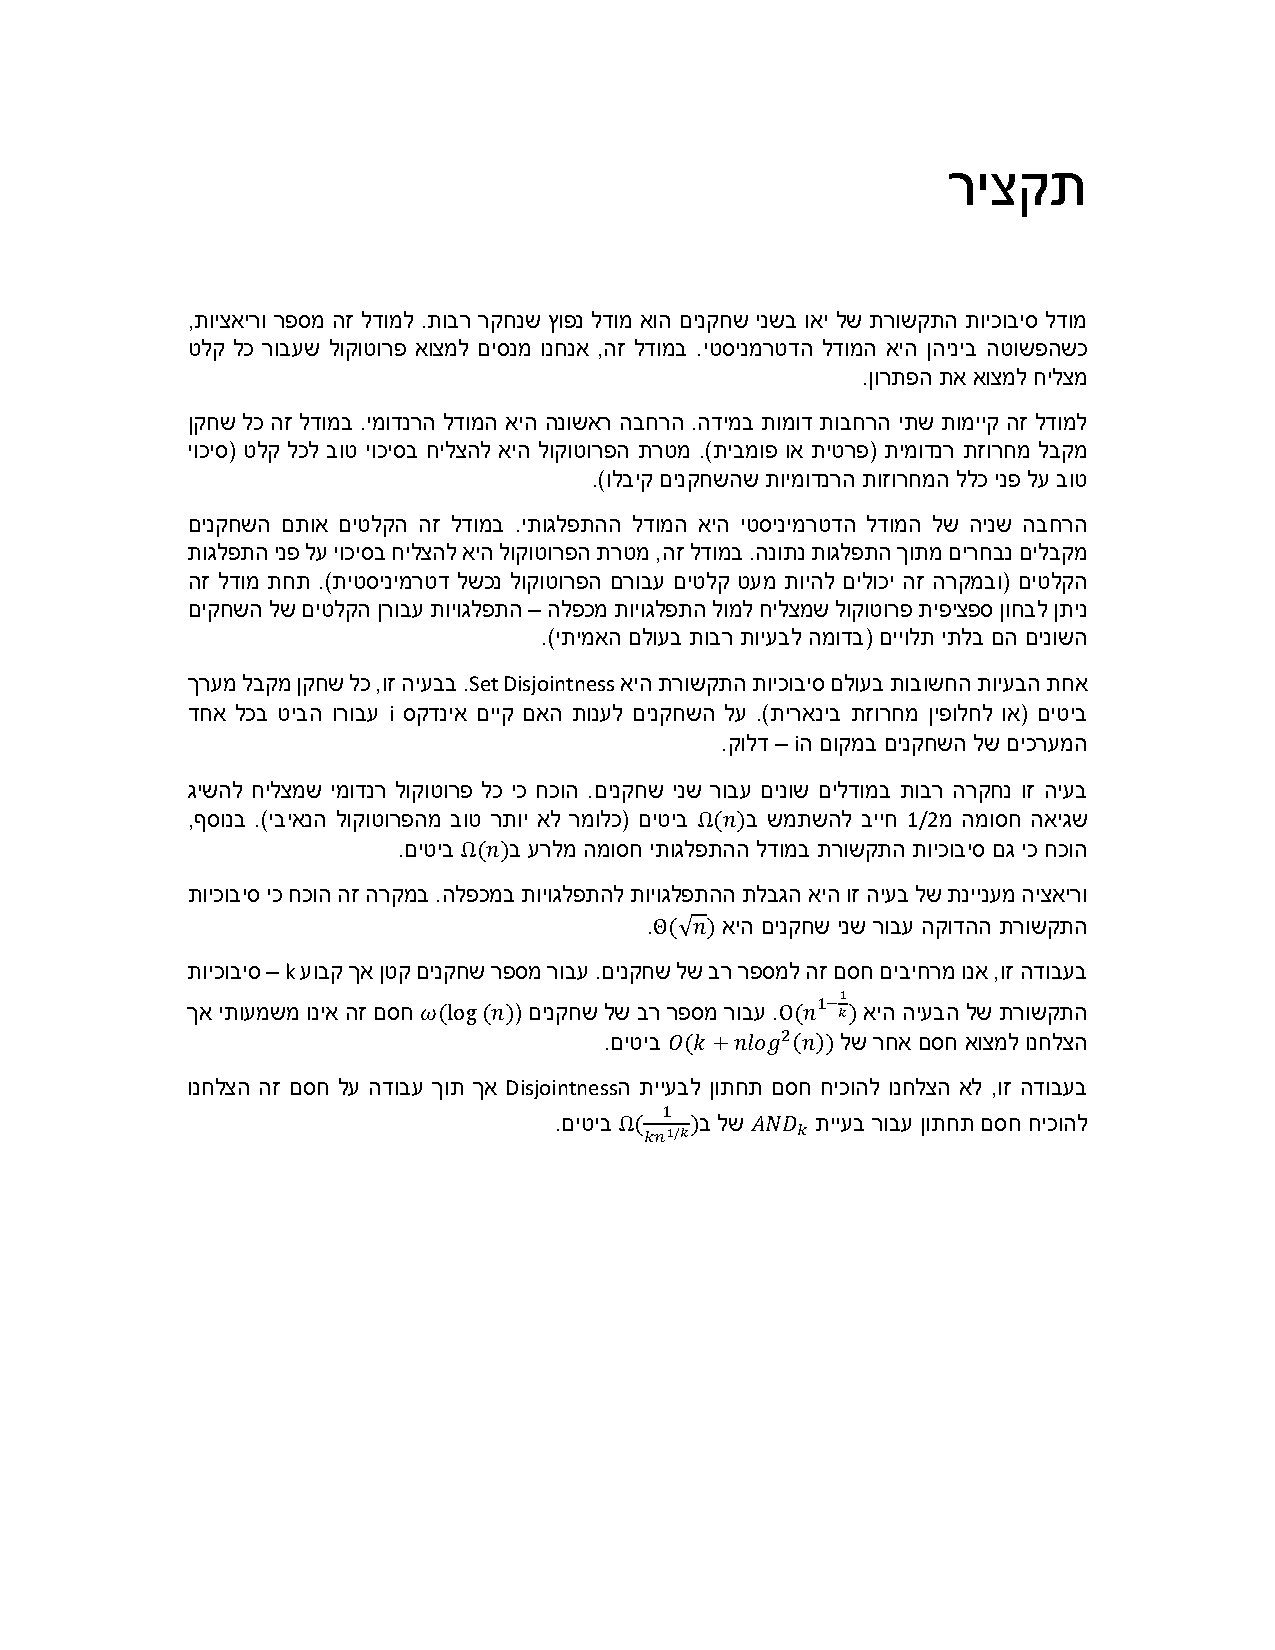
\includepdf[pages=-]{hebrew-abstract.pdf}

%% *** NOTE ***
%% If you don't use bibliography files, comment out the previous line
%% and use \begin{thebibliography}...\end{thebibliography}.  (In that
%% case, you should probably put the bibliography in a separate file and
%% `\include' or `\input' it here).

\end{document}